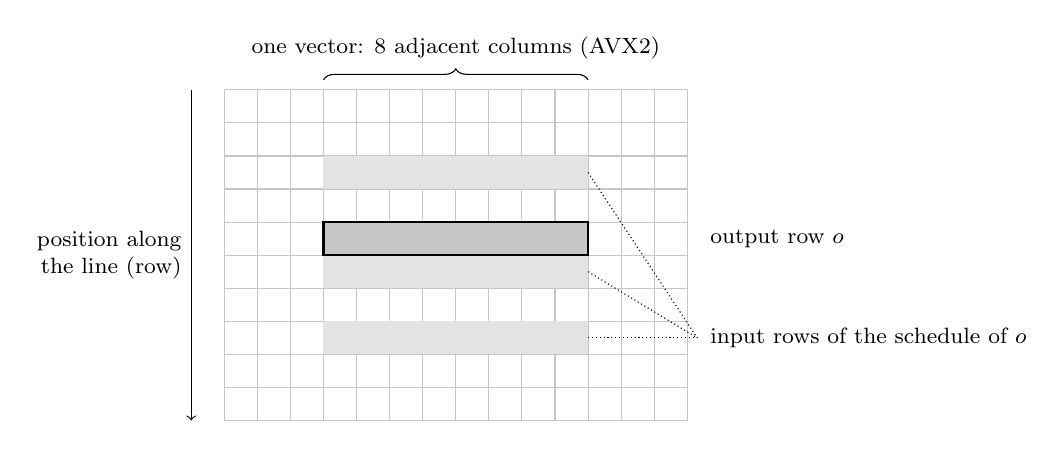
\begin{tikzpicture}[x=0.42cm,y=-0.42cm,font=\footnotesize]
  % a region: columns are lines of the column pass
  \foreach \c in {0,...,13} \foreach \r in {0,...,9} \draw[gray!45] (\c,\r) rectangle (\c+1,\r+1);
  \fill[gray!22] (3,2) rectangle (11,3);
  \fill[gray!22] (3,5) rectangle (11,6);
  \fill[gray!22] (3,7) rectangle (11,8);
  \fill[gray!45] (3,4) rectangle (11,5);
  \draw[line width=0.9pt] (3,4) rectangle (11,5);
  \draw[decorate,decoration={brace,amplitude=4pt}] (3,-0.3) -- (11,-0.3) node[midway,above=4pt] {one vector: 8 adjacent columns (AVX2)};
  \draw[->] (-1,0) -- (-1,10) node[midway,left,align=right] {position along\\the line (row)};
  \node[anchor=west] at (14.4,4.5) {output row $o$};
  \node[anchor=west] at (14.4,7.5) {input rows of the schedule of $o$};
  \draw[densely dotted] (11,2.5) -- (14.3,7.5);
  \draw[densely dotted] (11,5.5) -- (14.3,7.5);
  \draw[densely dotted] (11,7.5) -- (14.3,7.5);
\end{tikzpicture}
